\section{Деревья поиска}

\subsection{Двоичное дерево. Binary tree}
\begin{definition}[Двоичное дерево]
{\bfseries \scshape Двоичное дерево} определяется рекурсивно:
	\begin{enumerate}
		\item Либо оно пусто (не содержит вершин)
		\item Либо разбит на 3 непересекающиеся части: вершину, называемую {\bfseries корнем} (root), двоичное дерево, называемое {\bfseries левым поддеревом} (left subtree) корня, и двоичное дерево, называемое {\bfseries правым поддеревом} (right subtree) корня
	\end{enumerate}
	\cite{cormen}
\end{definition}
\par Примеры бинарных деревьев\par
\begin{enumerate}
	\item Обозначим белой вершинной - {\bfseries корень}, зелёным - {\bfseries левое поддерево}, красным - {\bfseries правое поддерево}\par
	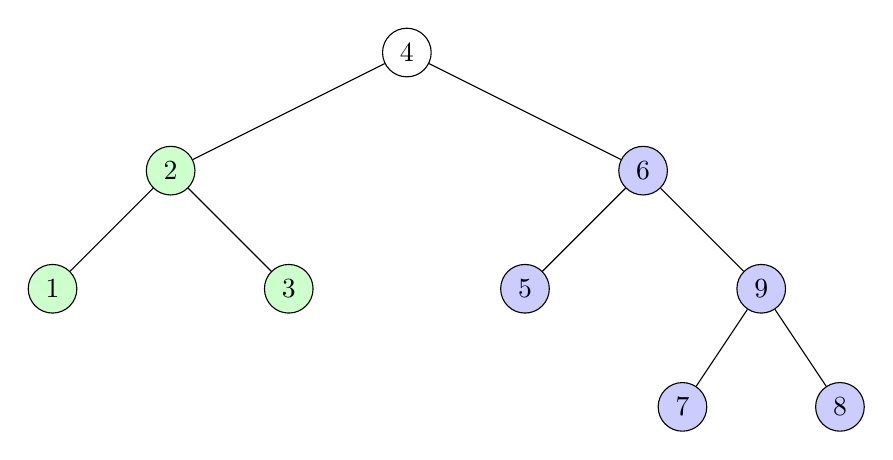
\begin{tikzpicture}[level/.style={sibling distance=60mm/#1}]
		\node [circle,draw] {4}
		child {
			node [fill=green!20,circle,draw] {2}
			child {node [fill=green!20,circle,draw] {1}
			}
			child {
				node [fill=green!20,circle,draw]{3}
			}
		}
		child {node [fill=blue!20,circle,draw] {6}
			child {node [fill=blue!20,circle,draw]  {5}
			}
			child {node [fill=blue!20,circle,draw]  {9}
				child {node [fill=blue!20,circle, draw]  {7}} 
				child {node [fill=blue!20,circle, draw]  {8}} 
			}
		};
	\end{tikzpicture}
	\item В данном случае правым поддеревом является пустым дерево \par
	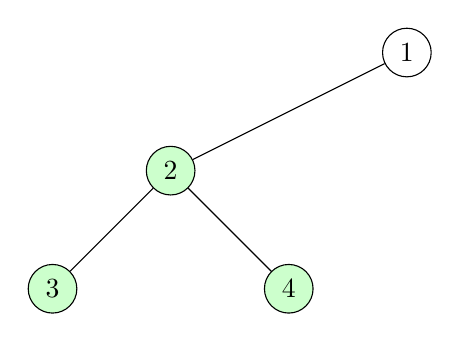
\begin{tikzpicture}[level/.style={sibling distance=60mm/#1}]
		\node [circle,draw] {1}
		child {node [fill=green!20,circle,draw] {2}
			child {node [fill=green!20,circle,draw]  {3}}
			child {node [fill=green!20,circle,draw]  {4}}
		}
		child [missing];
	\end{tikzpicture}
	\item Пустое бинарное дерево\par\par
\end{enumerate}

\newpage

\subsection{Двоичное дерево поиска. Binary search tree }
\begin{definition}[Двоичное дерево поиска]
	Двоичное дерево поиска- Это структура данных для работы с упорядоченными множествами.
\end{definition}
\begin{definition}[Свойство бинарного дерева поиска]
	Если x — узел бинарного дерева поиска, а узел y находится в левом
	поддереве x, то $key [y] \le  key [x]$. Если узел y находится в правом
	поддереве x, то $key [x] \le  key [y]$.
\end{definition}
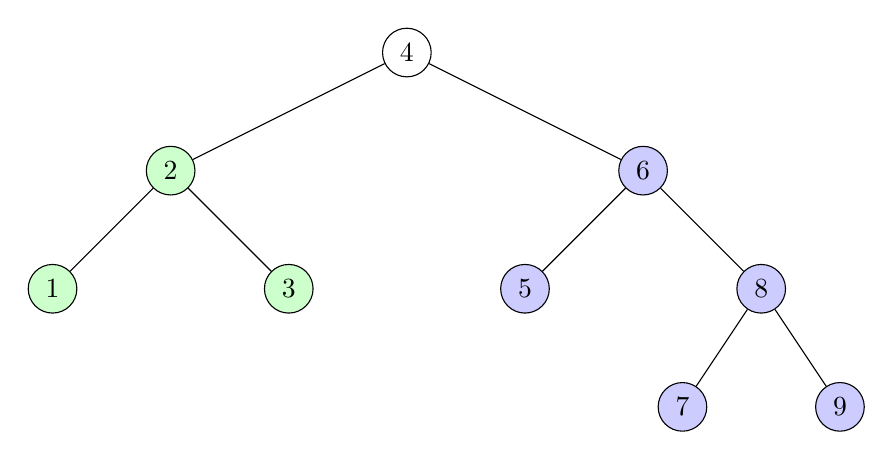
\begin{tikzpicture}[level/.style={sibling distance=60mm/#1}]
	\node [circle,draw] {4}
	child {
		node [fill=green!20,circle,draw] {2}
		child {node [fill=green!20,circle,draw] {1}
		}
		child {
			node [fill=green!20,circle,draw]{3}
		}
	}
	child {node [fill=blue!20,circle,draw] {6}
		child {node [fill=blue!20,circle,draw]  {5}
		}
		child {node [fill=blue!20,circle,draw]  {8}
			child {node [fill=blue!20,circle, draw]  {7}} 
			child {node [fill=blue!20,circle, draw]  {9}} 
		}
	};
\end{tikzpicture}\par

как мы можем видеть - все числа в зелённом поддереве меньше нашего корневого элемента и все элементы из правого больше корня $1,2,3 \le 4 \le 5,6,7,8,9$\par
это утверждение верно для каждого из поддеревьев нашего дерева\par
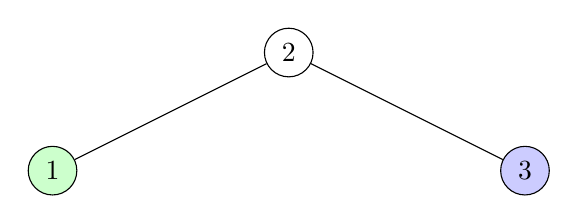
\begin{tikzpicture}[level/.style={sibling distance=60mm/#1}]
	\node [circle,draw] {2}
		child {node [fill=green!20,circle,draw] {1}
		}
		child {
			node [fill=blue!20,circle,draw]{3}
		};
\end{tikzpicture}
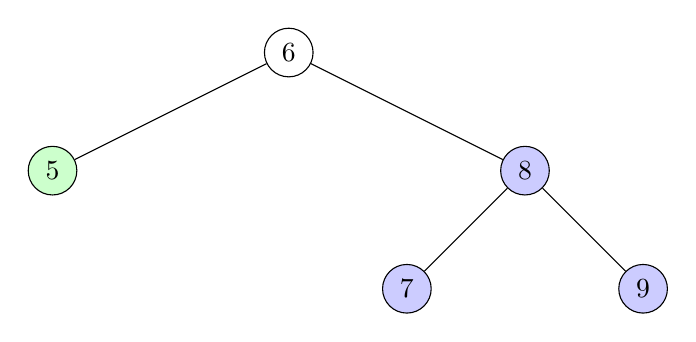
\begin{tikzpicture}[level/.style={sibling distance=60mm/#1}]
	\node [circle,draw] {6}
		child {node [fill=green!20,circle,draw]  {5}
		}
		child {node [fill=blue!20,circle,draw]  {8}
			child {node [fill=blue!20,circle, draw]  {7}} 
			child {node [fill=blue!20,circle, draw]  {9}} 
		};
	
\end{tikzpicture}\par
$1 \le 2 \le 3$ и $5 \le 6 \le 8,7,9$

\begin{note}
	У одного и того же множества ключей может существовать несколько построений бинарного дерева поиска
\end{note}\par
\begin{example}
	Покажем на примере набора $\left\{1,3, 5, 8, 12, 22,99\right\}$\par
	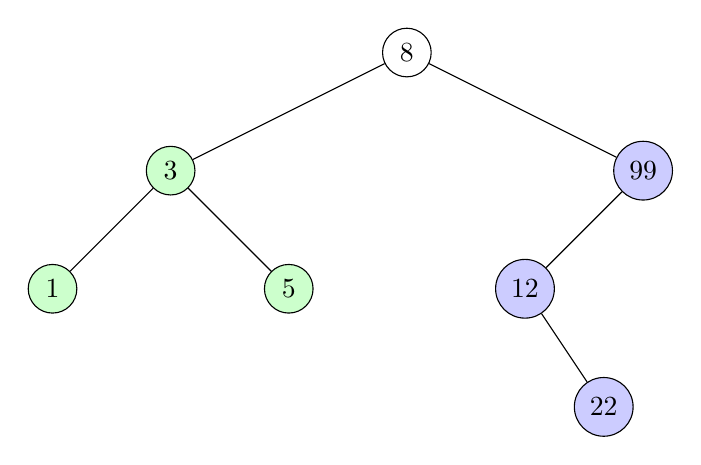
\begin{tikzpicture}[level/.style={sibling distance=60mm/#1}]
		\node [circle,draw] {8}
		child {node [fill=green!20,circle,draw]  {3}
			child {node [fill=green!20,circle, draw]  {1}} 
			child {node [fill=green!20,circle, draw]  {5}}
		}
		child {node [fill=blue!20,circle,draw]  {99}
			child {node [fill=blue!20,circle, draw]  {12}
				child [missing] 
				child {node [fill=blue!20,circle, draw]  {22}}
			} 
			child [missing]
		};
		
	\end{tikzpicture}
	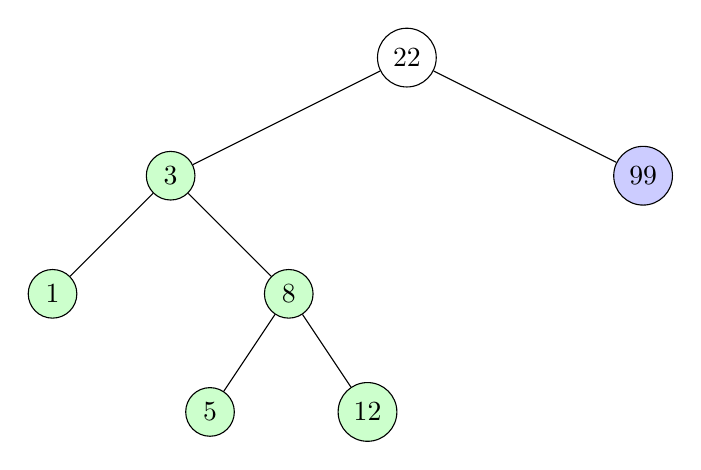
\begin{tikzpicture}[level/.style={sibling distance=60mm/#1}]
		\node [circle,draw] {22}
		child {node [fill=green!20,circle,draw]  {3}
			child {node [fill=green!20,circle, draw]  {1}} 
			child {node [fill=green!20,circle, draw]  {8}
				child {node [fill=green!20,circle, draw]  {5}} 
				child {node [fill=green!20,circle, draw]  {12}}
			}
		}
		child {node [fill=blue!20,circle,draw]  {99}};
		
	\end{tikzpicture}\par
\end{example}

\newpage

\subsection{Операции дерева поиска}

Двоичное дерево поиска позволяет нам выполнять нам следующие операции с динамическими множествами

\begin{enumerate}[]
	\item Поиск следующего и предыдущего элемента
	\item Min() и Max()	Поиск минимума и максимума
	\item Search(key)	Поиск элемента
	\item Inseart(key)
	\item Delete(key)
\end{enumerate}

\subsubsection{Search(X)}
по свойству бинарного дерева поиска нам известно, что Если x — узел бинарного дерева поиска, а узел y находится в левом
поддереве x, то $key [y] \le  key [x]$. Если узел y находится в правом
поддереве x, то $key [x] \le  key [y]$.

Тогда, если мы рассматриваем некоторую вершину $V$, возможны 3 варианта:\par
\begin{enumerate}[]
	\item $key[V]==X$\par
	тогда, очевидно, что мы нашли искомую вершину
	\item $key[V] \le X$\par
	тогда, вспоминая вышеописанное свойство, очевидно, что если наш элемент всё таки находится в дереве, то он должен находиться в правом поддереве нынешней вершины
	\item $key[V] \ge X$\par 
	тогда, наш элемент находиться в левом поддереве нынешней вершины
\end{enumerate}\par

Тогда наш алгоритм заключается...

\begin{example}
	
\end{example}

\subsubsection{Поиск минимума и максимума}
\subsubsection{Поиск следующего и предыдущего элемента}
\subsubsection{Inseart(key)}
\subsubsection{Delete(key)}

\newpage

\subsection{AVL Дерево}
Поскольку одному и тому же множеству можно построить несколько деревьев разной высоты,





